% (c) GreenSocs Ltd
% author: Christian Schroeder <schroeder@eis.cs.tu-bs.de>

\chapter{GreenControl Introduction}

This section contains a brief overview of the implementation ideas for the {\em GreenControl} project. The \GreenControl framework is extendable with \textsl{plugins} which provide a service and add new functionality. To minimize the effect on analysis tools as little as possible SystemC elements are used within \GreenControl and its extensions (since v. 4.1.0).

See the project page\footnote{\GreenControl project page:  \href{http://www.greensocs.com/projects/GreenControl}{http://www.greensocs.com/projects/GreenControl}} for further documentation and downloads.

\section{Transaction-based approach}

The \GreenControl framework is based on a transaction-based approach. The \GreenControl Core is a router that connects user modules with service providers (plugins).
\begin{itemize}
	\item The connections are established via ports (but not using SystemC ports).
	\item Communication takes place using a special extendable transaction container.
\end{itemize}


\begin{figure}[htbp]
	\centerline{
		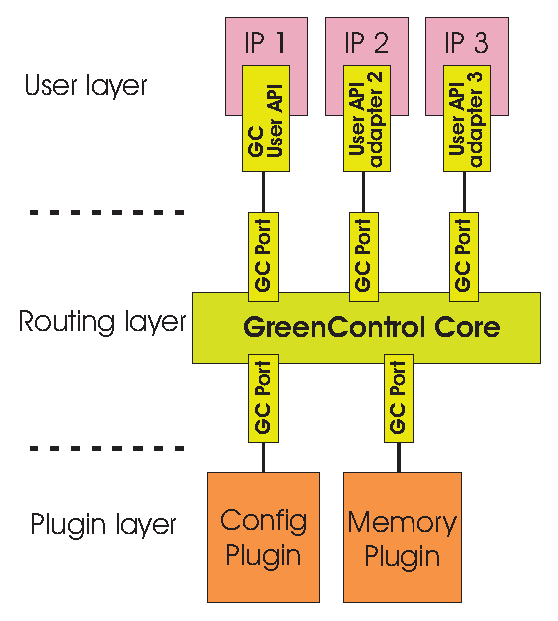
\includegraphics[width=10cm]{GreenControl.eps}} 
	\caption{GreenControl framework with service plugins.}
	\label{fig:GreenControl}
\end{figure}

Figure \ref{fig:GreenControl} shows the approach. The \GreenControl Core routes transactions between the IPs and plugins. One or more of the IPs may be a tool.



\section{Transaction container}
A transaction container contains generic attributes to transfer commands between the user modules and the service providers. The concepts of {\em atoms} and {\em quarks} in the \GreenBus transaction container will be adopted. 

\noindent
\begin{minipage}{\textwidth}
Example: 

\begin{tabular}{|l|}
	\cline{1-1} Service = ConfigService   \\ 
	\cline{1-1} Target = top.jpeg.compression\_rate   \\ 
	\cline{1-1} Command = setParam   \\ 
	\cline{1-1} Value = 42   \\ 
	\cline{1-1} ...   \\ 
	\hline
\end{tabular}
\end{minipage}

Advantages of this approach are 
\begin{itemize}
	\item decoupling of config APIs and config implementation 
	\item well-defined protocol with clear semantics 
	\item easy to add new commands 
	\item easy to add new services, e.g. address management, memory framework, debug fabric, ... 
	\item dynamic extension mechanism
\end{itemize}


\section{GreenControl Core}
The Core forwards transactions from the initiator to the target. For the above example, the target would be a ConfigPlugin. Upon receipt of the transaction, the ConfigPlugin would process the service request {\em setParam("top.jpeg.compression\_rate", 42)} and acknowledge the transaction. 

\begin{itemize}
	\item Flexibility: Service providers (plugins) and user modules can be attached at elaboration time, without the need for re-compilation of the model. 
	\item Reliability: if a service is requested that is not available/implemented by the service provider, the transaction can be rejected and a warning generated.
	\item Debugging: all transactions can be monitored in order to trace usage of the \GreenControl services.
\end{itemize}



\section{User APIs}
User APIs are the APIs the user module sees and interacts with. They provide some functionality to the user module (IP). User APIs are connected to the \GreenControl Core with a port (GC Port). They send transactions to the one service plugin which belongs to their functionality and task.

\begin{itemize}
	\item APIs provide methods whose calls are translated into the appropriate \GreenControl transactions. 
	\begin{itemize}
		\item Simple API methods such as setParam/getParam can be directly translated into a transaction.
		\item More complex API method calls may require some housekeeping.
	\end{itemize}

	\item User APIs receive transactions from the plugin and process them.
\end{itemize}


\section{Plugins}
Plugin are the service providers for the \GreenControl framework. Different plugins may provide different functionality, such as configuration, analysis, visibility, memory and address management, debugging etc.

Thus, \GreenControl is a versatile base fabric for the implementation of SystemC extension frameworks.

Existing plugins are the {\em configuration service plugin} \GreenConfig\footnote{\GreenConfig project page:  \href{http://www.greensocs.com/projects/GreenControl/GreenConfig}{http://www.greensocs.com/projects/GreenControl/GreenConfig}} and the {\em analysis and visibility service plugin} \GreenAV\footnote{\GreenAV project page:  \href{http://www.greensocs.com/projects/GreenControl/GreenAV}{http://www.greensocs.com/projects/GreenControl/GreenAV}}. 



\section{Additional information}

The SystemC model only needs to include the used plugins. When e.g. memory management isn't needed, this plugin can be left out. The connection is done automatically during instantiation, hence no recompiling is needed if the usage of a plugin is changed. 

The communication through ports and universal transaction containers gives the ability to extend \GreenControl without changing the Core itself. 

Newly developed plugins can be connected with the standard port without changing the \GreenControl Core. So this extension can even done by a user. 

To give the ability of extending \GreenControl the transaction
container has to be either very general to be useful in a new
developed plugin or it has to be extendable itself. The extension of
the container could be done by simple inheritance. 
The transmission of a transaction is more complex (and more time consuming) than simple method calls.
